%\documentclass[12pt,a4paper]{report}
\documentclass[12pt,a4paper,oneside,onecolumn,openright]{book}
% set the document language
\usepackage[italian]{babel}
% set the encoding used by your editor here (default is utf8)
\usepackage[utf8]{inputenc}
\usepackage[T1]{fontenc}

% math packages
\usepackage{amsmath}
\usepackage{amssymb}
\usepackage{lmodern}
\usepackage{varwidth}
\usepackage{xcolor}
\usepackage[makeroom]{cancel}
% page margins settings
\usepackage[inner=1.5cm,outer=1.5cm,top=1.5cm,bottom=1.5cm]{geometry}
%\usepackage{indentfirst}

% other packages
\usepackage{array}
\usepackage{enumitem}
\usepackage{subfigure}
\usepackage{graphicx}
\usepackage{verbatim}
\usepackage{listings}
\usepackage{url}
\usepackage[hidelinks]{hyperref}
\usepackage[export]{adjustbox}
\usepackage{latexsym}
\usepackage{tabularx}
\usepackage{ragged2e}
\usepackage{mathtools}
\DeclarePairedDelimiter\floor{\lfloor}{\rfloor}
\DeclarePairedDelimiter\ceil{\lceil}{\rceil}
% \usepackage{Mathematics}
% custom colors
\usepackage{color}
\usepackage{wrapfig}
\usepackage{gensymb}
\usepackage{caption}
\usepackage{tikz}
\usepackage{forest}
\usepackage{tikz-qtree}

\newcommand\myeq{\stackrel{\mathclap{\tiny\mbox{def}}}{=}}

\usepackage[many]{tcolorbox}
\newtcolorbox{boxA}{
    % fontupper = \bf,
    boxrule = 1.5pt,
    colframe = black % frame color
}

\usetikzlibrary{shadows}
\definecolor{light-gray}{gray}{0.96}
\definecolor{cyan}{RGB}{230,230,255}
\definecolor{dkgreen}{rgb}{0,0.6,0}
\definecolor{gray}{rgb}{0.5,0.5,0.5}
\definecolor{mauve}{rgb}{0.58,0,0.82}
\definecolor{iceberg}{rgb}{0.44, 0.65, 0.82}
% \definecolor{blue}{RGB}{44, 44, 210}

\hypersetup{
colorlinks=true,
linkcolor=black,
% filecolor=blue,
urlcolor=blue,
% pdftitle={Overleaf Example},
}

\urlstyle{same}
\graphicspath{ {./images/} }

% environment for bash code
\lstset{ %
  language=bash,                % the language of the code
  basicstyle=\footnotesize,           % the size of the fonts that are used for the code
  numbers=left,                   % where to put the line-numbers
  numberstyle=\footnotesize,          % the size of the fonts that are used for the line-numbers
  stepnumber=1,                   % the step between two line-numbers. If it's 1, each line 
                                  % will be numbered
  numbersep=5pt,                  % how far the line-numbers are from the code
  backgroundcolor=\color{white},      % choose the background color. You must add \usepackage{color}
  showspaces=false,               % show spaces adding particular underscores
  showstringspaces=false,         % underline spaces within strings
  showtabs=false,                 % show tabs within strings adding particular underscores
%  frame=single,                   % adds a frame around the code
  rulecolor=\color{black},        % if not set, the frame-color may be changed on line-breaks within not-black text (e.g. commens (green here))
  tabsize=2,                      % sets default tabsize to 2 spaces
  captionpos=b,                   % sets the caption-position to bottom
  breaklines=true,                % sets automatic line breaking
  breakatwhitespace=false,        % sets if automatic breaks should only happen at whitespace
  title=\lstname,                   % show the filename of files included with \lstinputlisting;
                                  % also try caption instead of title
  numberstyle=\tiny\color{gray},        % line number style
  keywordstyle=\textbf,          % keyword style
  commentstyle=\color{dkgreen},       % comment style
%  stringstyle=\color{mauve},         % string literal style
  escapeinside={\%*}{*)},            % if you want to add a comment within your code
  morekeywords={*,...,insert,-}               % if you want to add more keywords to the setù
}

% environment for python code
\lstset{
	language=Python,
	breaklines=true,
	breakatwhitespace=true ,
	backgroundcolor=\color{light-gray}
}

\newcommand{\grayScale}{0.95} % Can change the gray level here
\definecolor{codeBackground}{rgb}{\grayScale ,\grayScale ,\grayScale}
\definecolor{forestGreen}{rgb}{0.13,0.55,0.13}

\lstset{
    language=C,
    backgroundcolor=\color{codeBackground},
    tabsize=4,
    showstringspaces=false,
    showtabs=false,
    showspaces=false,
    basicstyle=\ttfamily,
    identifierstyle=\ttfamily,
    keywordstyle=\color{blue},
    stringstyle=\color{red},
    commentstyle=\color{gray},
    numberstyle=\color{magenta},
    morecomment=[l][\color{forestGreen}]{\#},
    escapechar={|}, 
}
% appendices package
%\usepackage{appendix}
% set Appendix name used in the toc
%\renewcommand{\appendixtocname}{Appendice}

% interline
\linespread{1.5}
% set numbers for subsections and show them in the toc
\setcounter{tocdepth}{3} 
\setcounter{secnumdepth}{3}

% layout package, style and settings
\usepackage{fancyhdr}
\pagestyle{fancy}

\fancypagestyle{mainmatter}{%		
		\fancyhf{} 
		\fancyhead{}
		\fancyhead[LE,RO]{\thepage}
		\fancyhead[LO]{\footnotesize{\leftmark}}
		\fancyhead[RE]{\footnotesize{\rightmark}}
		\fancyfoot{}
		\addtolength{\headwidth}{\marginparsep}
		\addtolength{\headheight}{2.5pt}
		\renewcommand{\headrulewidth}{0.3pt}
		\renewcommand{\footrulewidth}{0.0pt}
		}
\fancypagestyle{frontmatter}{%
		\fancyhf{} 
		\fancyhead[LE]{\footnotesize{\MakeUppercase{\thepage}}}
		\fancyhead[RO]{\footnotesize{\MakeUppercase{\thepage}}}
		\fancyhead[RE,LO]{}
		\fancyfoot{}
		\addtolength{\headwidth}{\marginparsep}
		\addtolength{\headheight}{2.5pt}
		\renewcommand{\headrulewidth}{0.0pt}
		\renewcommand{\footrulewidth}{0.0pt}
		}
		
		
\usepackage{fancyhdr}
\pagestyle{fancy}
		\fancyhf{} 
		\fancyhead{}
		\fancyhead[LE,RO]{\thepage} 
		\fancyhead[LO]{\footnotesize{\leftmark}}
		\fancyhead[RE]{\footnotesize{\rightmark}}
		\fancyfoot{}
		\addtolength{\headwidth}{\marginparsep}
		\addtolength{\headheight}{2.5pt}
		\renewcommand{\headrulewidth}{0.3pt}
		\renewcommand{\footrulewidth}{0.0pt}

% empty pages have no numbers
\makeatletter
\def\cleardoublepage{\clearpage\if@twoside \ifodd\c@page\else
\hbox{}
  %Potresti voler togliere il commento dalla linea seguente
  %Questa pagina � stata lasciata intenzionalmente vuota.
\thispagestyle{empty}
\newpage
\if@twocolumn\hbox{}\newpage\fi\fi\fi}
\makeatother
%????
%\textwidth=450pt\oddsidemargin=0pt

%\makeatletter 
%  \DeclareRobustCommand*\textsubscript[1]{% 
%    \@textsubscript{\selectfont#1}} 
%  \newcommand{\@textsubscript}[1]{% 
%    {\m@th\ensuremath{_{\mbox{\fontsize\sf@size\z@#1}}}}} 
\makeatother 

\begin{document}
\begin{titlepage}
\begin{center}
{
    \large
    \textbf{Università  degli studi di Modena e Reggio Emilia} \\
   	\textbf{Dipartimento di Ingegneria Enzo Ferrari} \\
    \vspace{\stretch{0.5}}
    \hspace*{0cm} \hrulefill \hspace*{0cm} \\
    \vspace{\stretch{0.5}}    
	  \vspace{\stretch{12}}
  
  
 		\huge{\bf Matematica Discreta }}\\
		\vspace{3mm}
		
		\vspace{\stretch{6}}
		\end{center}
		
\vspace{40mm}
\par
\noindent
\vspace{20mm}
\begin{center}
\hspace*{0cm} \hrulefill \hspace*{0cm} \\
{\large{\bf 
Anno Accademico 2023/24}}
\end{center}

\end{titlepage}

\pagestyle{frontmatter}
\frontmatter

% PAGINA VUOTA
%\clearpage\null\thispagestyle{empty}\clearpage
\setcounter{tocdepth}{2}
\tableofcontents

\setlength{\parindent}{12pt}
\setlength{\parskip}{1ex plus 0.5ex minus 0.2ex}
\mainmatter
\pagestyle{mainmatter}

\chapter{Introduction}

\section{Structure and Content}
\begin{itemize}

    \item \textbf{Module 1}: 
    \begin{enumerate}
        \item \textbf{\textit{intra-vehicles communications}}: nodes, sensors, ECU
        \item \textbf{\textit{signal busses}}: CAN, LIN, FlexRay, MOST, Ethernet [ T1/T1S]
        \item \textbf{\textit{car domain and OS}}
    \end{enumerate}
    
    \item \textbf{Module 2}:
    \begin{enumerate}
        \item \textbf{\textit{inter-vehicles communications}}: \textit{V2V} and \textit{V2X} (car is a node)
        \item \textbf{\textit{wireless technologies}}: Bluetooth, LoRa, C-V2X, IEE 802.11p (bd)
        \item application, messages, broadcast, GPS
    \end{enumerate}

\end{itemize}
Different \textbf{domain} or \textbf{application} needs different \textit{communications protocols}, is important to understand how each nodes in domain communicate each other (inside the car).

\newpage
\section{Intra-Vehicles}
From the 80's, where the car's control unit are isolated an there was a dedicated wires connect sensors and actuators with less electronic than now, until the reach the greates goal of evolution in the automotive sector: autonomous drive. The complexity of the number of connection from each ECU's to the other, also the number of ECU's for each car, is growing. While the number of signal increase in a liner way, the connection between ECU's is growing with a quadratic complexity $O(n^2)$.

If we examine the evolutions of the ECUs number inside an ``Audi A6'' we can observe that in 1997 it has 5 ECUs and in the 2007 it has 50 ECUs, instead the ``Tesla M3'' in the 2017 has 70 ECUs. The quadratic increase of ECUs number, however has reach a cap for two main reason: the cost and the space inside the car. Traditionally one ECUs is responsible of one task, but nowadays it could be two type of trends:
\begin{enumerate}[nosep]
    \item \textit{distributed of function across ECUs}
    \item \textit{integration of multiple function in one ECU}
\end{enumerate}

\section{Architectures}

\begin{figure}[h]
    \centering
    \begin{minipage}[t]{0.45\textwidth}
        \centering
        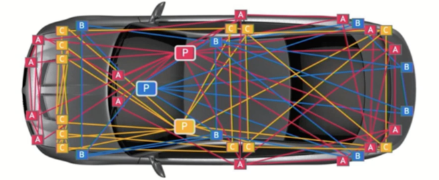
\includegraphics[width=\textwidth]{img/domain_architecture}
        \caption{\textit{Domain Architecture}}
        
        \begin{flushleft}
            \begin{enumerate}[nosep]
                \item central domain controller (\textbf{P}) or high performance computer
                \item ability to handle more complex functions
                \item cost optimization
                \item cable harness is rigid and expensive
            \end{enumerate}
        \end{flushleft}

    \end{minipage}
    \begin{minipage}[t]{0.45\textwidth}
        \centering
        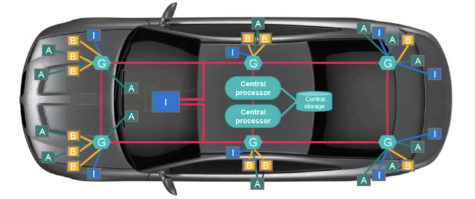
\includegraphics[width=\textwidth]{img/zonal_architecture}
        \caption{\textit{Zonal Architecture}}
        
        \begin{flushleft}
            \begin{enumerate}[nosep]
                \item local ethernet per zone (\textbf{G})
                \item ultra high-speed secured backbone between zone
                \item centralized software
                \item central computer storage
            \end{enumerate}
        \end{flushleft}
        
    \end{minipage}
\end{figure}
\chapter{Parte 3}
\section{Strutture algebriche elementari}
Una \textbf{operazione binaria intera} su un insieme G è un'applicazione 
\begin{center}
    $\ast \; : \; G \times G \rightarrow G$
\end{center}
L'immagine della coppia $(x,y)$ si denoterà con $x \ast y$. 
\begin{itemize}
    \item $e \in G$ si dice \textbf{elemento neutro} rispetto a $\ast$ se:
    \begin{center}
        $g \ast e = e \ast g = g \; \forall g \in G$
    \end{center}
    \item un elemento $g \in G$ si dice invertibile se esiste $\bar{g} \in G$ tale che $g * \bar{g} = \bar{g} * g = e$
\end{itemize}

\subsection{Gruppi}
La coppia $(G, \ast)$, con $\ast$ operazione su G, si dice \textbf{gruppo} se vengono rispettate le seguenti proprietà:
\begin{itemize}
    \item $\ast$ è \textbf{associativa}: $\forall g, g', g'' \in G$ si ha $(g \ast g') \ast g'' = g \ast (g' \ast g'')$
    \item esiste l'elemento \textbf{neutro}
    \item ogni elemento di G è invertibile
\end{itemize}
Il gruppo si dice \textbf{abeliano} o \textbf{commutativo} se: 
\begin{center}
    $\forall g, g' \in G, \; g \ast g' = g' \ast g$ (proprietà \textbf{commutativa})
\end{center}
Alcuni \textcolor{yellow}{\textbf{esempi}}:
\begin{itemize}
    \item $(\mathbb{N}, +)$, $(\mathbb{Z}, \cdot)$ non sono gruppi. in quanto non né in $\mathbb{N}$ e $\mathbb{Z}$ sono presenti per ogni elemento dell'insieme dell'elemento inverso, in $\mathbb{N}$ non sono presenti elementi negativi, quindi nessun elemento avrà un'altro che sommato a se stesso dia 0, viceversa l'insieme $\mathbb{Z}$ che sono presenti elementi positivi e negativi viene definita l'operazione $\cdot$ richiede i reciproci dei singoli elementi affiché possano essere definiti gli elementi inversi.
    \item $(\mathbb{Z}, +)$, $(\mathbb{Q}, \cdot)$ sono gruppi abelliani
\end{itemize}

\subsection{Anelli}
La terna $(\mathbb{A}, +, \cdot)$ con $\mathbb{A}$ un insieme e $+, \cdot$ (somma e prodotto) due operazione binarie interne a $\mathbb{A}$, si dice \textbf{anello} se:
\begin{itemize}
    \item $(\mathbb{A}, +, \cdot)$ è un gruppo \textbf{abeliano} (con elemento neutro 0).
    \item il prodotto è \textbf{associativo}.
    \item per ogni $x,y,z \in \mathbb{K}$ si ha $x \cdot (y + z) = (x \cdot y) + (x \cdot z)$ e $(x + y) \cdot z = (x \cdot z) + (y \cdot z)$ (il prodotto è distribuito rispetto alla somma).
\end{itemize}
Un anello $(\mathbb{A}, +, \cdot)$ è detto \textbf{commutativa} se il prodotto è commutativo, mentre è detto \textbf{unitario} o con \textbf{unità} se $(\mathbb{A}, \cdot)$ ammette l'elemento neutro. $(\mathbb{Z}, +, \cdot)$, $(\mathbb{Q}, +, \cdot)$, $(\mathbb{R}, +, \cdot)$, $(\mathbb{C}, +, \cdot)$ sono anelli.

\newpage
\subsection{Campi}
La terna $(\mathbb{K}, +, \cdot)$ con $\mathbb{K}$ un insieme e $+, \cdot$ (somma e prodotto) due operazioni binarie interne a $\mathbb{K}$, si dice \textbf{campo} se:
\begin{itemize}
    \item $(\mathbb{K}, +)$ è un gruppo \textbf{abeliano} (con elemento neutro 0).
    \item $(\mathbb{K} - \{0\}, \cdot)$ è un gruppo \textbf{abeliano} (con elemento neutro 1).
    \item per ogni $x,y,z \in \mathbb{K}$ si ha $x \cdot (y + z) = (x \cdot y) + (x \cdot z)$ quindi il prodotto è distribuito rispetto alla somma.
\end{itemize}
In qualunque campo vale la \textbf{legge di annullamento del prodotto}:
\begin{center}
    $x \cdot y = 0 \rightarrow x = 0 \; \text{oppure} \; y = 0$
\end{center}

\subsection{Domini d'integrità}
\textbf{Divisori dello zero}: sia $(A, +, \cdot)$ un anello. Due elementi $a,b \in A$ si dicono \textbf{divisori dello zero} se $a \neq 0$, $b \neq 0$, ma $a \cdot b = 0$. Ad \textcolor{yellow}{\textbf{esempio}} l'anello delle matrici quadrate presenta dei divisori dello zero. \\
Un anello commutativo privo di divisori dello zero si dice \textbf{dominio di integrità}, ad \textcolor{yellow}{\textbf{esempio}} $(\mathbb{Z}, +, \cdot)$ è un anello commutativo unitario privo di divisori dello zero. Quindi è dominio di integrità.

\section{L'anello dei numeri interi}
È noto che $\exists h \; | \; h : \mathbb{Z} \rightarrow \frac{\mathbb{N}_0 \times \mathbb{N}_0}{\mathcal{R}}$ dove la relazione di equivalenza che si vuole definire è $\equiv_n$. Su questo insieme vengono \textbf{ben poste} le seguenti operazioni:
\begin{center}
    $\boxplus : \mathbb{Z} \times \mathbb{Z} \rightarrow \mathbb{Z}$ \\
    $((m, n), (m', n')) \mapsto [(m, n)] \boxplus [(m', n')] \myeq [(m + m', n + n')]$

    $\boxdot : \mathbb{Z} \times \mathbb{Z} \rightarrow \mathbb{Z}$ \\
    $((m, n), (m', n')) \mapsto [(m, n)] \boxdot [(m', n')] \myeq [(mm' + nn', mn' + m'n)]$
\end{center}
Definito questo possiamo dire che $(\mathbb{Z}, \boxplus, \boxdot)$ è \textbf{dominio di integrità}.

\section{Teoria della Divisibilità}
\textbf{Divisibilità}: dati due numeri $a,b \in \mathbb{Z}$, si dice che $a$ \textbf{divide} $b$ (e si scrive $a|b$) se:
\begin{center}
    $\exists c \in \mathbb{Z} \; | \; b = a \cdot c$
\end{center}
\textbf{Transitività}: se $n|m$ e $m|q$ allora $n|q$. \\
\textcolor{green}{\textbf{Dimostrazione}}: per ipotesi $\exists h \in \mathbb{Z} \; | \; m = h \cdot n$ e $\exists h' \in \mathbb{Z} \; | \; q = h' \cdot m$. Sostituendo la prima relazione nella seconda si ottiene $q = h' \cdot h \cdot n$. Poichè $h' \cdot h \in \mathbb{Z}$ abbiamo definito che $n|q$. \\ \newline
Se $n|m$ e $m|n$, allora $m \pm n$. \\
\textcolor{green}{\textbf{Dimostrazione}}: per ipotesi $\exists h \in \mathbb{Z} \; | \; m = h \cdot n$ e $\exists h' \in \mathbb{Z} \; | \; n = h' \cdot m$ andiamo a sostituire la seconda alla prima equazione:
\begin{center}
    \begin{align*}
        n &= h' \cdot h \cdot m \\
        n - h' \cdot h \cdot m &= 0 \\
        n \cdot (1 - h' \cdot h) &= 0
    \end{align*}
\end{center}
Essendo che $\mathbb{Z}$ è un \textbf{dominio di integrità}, segue che o $n = 0$ oppure $(1 - h' \cdot h) = 0 \rightarrow (h' \cdot h) = 1$, consideriamo che $n \leq 0$ e che quindi $h' \cdot h = 1$ sappiamo che $h$ ammette un inverso $h'$, da cui $h = h' = 1$ o $h = h' = -1$ (in $\mathbb{Z}$, gli unici elementi che ammettono inverso sono $1$ e $-1$). In questo modo sappiamo che $m=n$ oppure $m=-n$.

\section{Massimo Comune Divisore}
Dati $a,b \in \mathbb{Z}$ non entrambi nulli, si dice che $d \in \mathbb{Z}$ è \textbf{UN massimo comune divisore} tra $a$ e $b$ se:
\begin{itemize}
    \item $d|a$ e $d|b$
    \item $\forall d' \in \mathbb{Z} \; | \; d'|a, \; d'|b \Rightarrow d'|d$
\end{itemize}
Se $d$ e $d'$ sono due massimi comuni divisori tra $a$ e $b$ allora $d' = \pm d$.
\chapter{Aritmetica Modulare}
È nota la definizione di \textbf{insieme delle classi resto modulo $n$} $\mathbb{Z}_n \; (\forall n \in \mathbb{N}, n \geq 2)$, come insime quoziente di $\mathbb{Z}$ rispetto alla \textbf{relazione di congruenza} modulo $n$:

{\centering
    $a \equiv_n b \Longleftrightarrow \exists h \in \mathbb{Z} \; \text{t.c.} \; b - a = h \cdot n$
\par}
Inoltre:

{\centering
    $\mathbb{Z}_n = \frac{\mathbb{Z}}{\equiv_n} = \{[0], [1], ..., [n-1]\}$
\par}

\section{Operazioni in $\mathbb{Z}_n$}
Su $\mathbb{Z}_n = \frac{\mathbb{Z}}{\equiv_n}$ sono ben poste la \textbf{somma} e il \textbf{prodotto}

\subsection{Somma in $\mathbb{Z}_n$}

{\centering
    $\boxplus : \mathbb{Z}_n \times \mathbb{Z}_n \mapsto \mathbb{Z}_n$ \\
    $([a], [b]) \mapsto [a] \boxplus [b] \overset{\text{def}}{=} [a + b]$
\par}

\begin{boxA}
    \textcolor{olive}{\textbf{Dimostrazione}}: per provare che la somma è ben posta, occorre provare che, $\forall a' \in [a]$ e $\forall b' \in [b]$, si ha $[a' + b'] = [a + b]$. \\ 
    Per \textbf{Hp.} avremo che $\exists h \in \mathbb{Z} \; \text{t.c.} \; a' - a = h \cdot n$ ed $\exists h' \in \mathbb{Z} \; \text{t.c.} \; b' - b = h' \cdot n$. Facendo la somma otteniamo:

    {\centering
        $(a' - a) + (b' - b) = (h' \cdot n) + (h \cdot n)$ \\
        $(a' + b') - (a + b) = n \cdot \underset{\in \mathbb{Z}}{\fcolorbox{red}{white}{$(h' - h)$}}$
    \par}
    In questo modo siamo riusciti a provare la nostra \textbf{Th.}
\end{boxA}

\subsection{Prodotto in $\mathbb{Z}_n$}

{\centering
    $\boxdot : \mathbb{Z}_n \times \mathbb{Z}_n \mapsto \mathbb{Z}_n$ \\
    $([a], [b]) \mapsto [a] \boxdot [b] \overset{\text{def}}{=} [a \cdot b]$
\par}

\begin{boxA}
    \textcolor{olive}{\textbf{Dimostrazione}}: per provare che il prodotto è ben posto, occorre provare che $\forall a' \in [a]$ e $\forall b' \in [b]$, si ha $[a' \cdot b'] = [a \cdot b]$. \\
    Per \textbf{Hp.} avremo che $\exists h \in \mathbb{Z} \; \text{t.c.} \; a' - a = h \cdot n$ ed $\exists h' \in \mathbb{Z} \; \text{t.c.} \; b' - b = h' \cdot n$. Moltiplicando membro a membro $a' = a + hn$ e $b' = b + h'n$ otteniamo:

    {\centering
        $a' \cdot b' = (a + hn) \cdot (b + h'n) = ab + ah'n + bhn + hh'n^2$ \\
        $a'b' - ab = ah'n + bhn + hh'n^2 = n \cdot (\underset{\in \mathbb{Z}}{\fcolorbox{red}{white}{$ah' + bh + hh'n$}})$
    \par}
    In questo modo siamo riusciti a provare la nostra \textbf{Th.}
\end{boxA}

\begin{flushleft}
    \textbf{Proposizione}: $(\mathbb{Z}_n, \boxplus, \boxdot)$ è un anello commutativo con unità, $\forall n \in \mathbb{N}, n \geq 2$ 

    \textbf{Teorema}: $(\mathbb{Z}_n, \boxplus, \boxdot)$ è un campo \textit{se e solo se} $n$ è \textbf{primo}.

    \begin{boxA}
        \textcolor{olive}{\textbf{Dimostrazione}}
        
        \textcolor{red}{\textbf{Prima Parte}} ``$\Rightarrow$'': se $n$ non è primo avremo che $n = a \cdot b, \; \text{con} \; \{a, b\} \neq \{n, 1\}$ ma allora in $\mathbb{Z}_n$ avremo che $[a] \cdot [b] = [a \cdot b] = n = [0]$ il che significa che $\mathbb{Z}_n$ ammette divisori dello zero e quindi non può essere un campo.

        \textcolor{red}{\textbf{Seconda Parte}} ``$\Leftarrow$'': se $n$ è primo, bisogna dimostrare che ogni elemento non nullo ammette l'inverso. Si può dire che $[a] \neq [0] \Rightarrow a \not \equiv_n 0$ quindi che $a$ non è multiplo di $n$.

        Quindi il $\gcd (a, n) = 1$, quindi per l'\textbf{identità di bezout} $\exists \alpha, \beta \in \mathbb{Z} \; \text{t.c.} \; 1 = \alpha \cdot a + \beta \cdot n$ che si può riscrivere come:

        {\centering
            $1 - \underset{\in [1]}{\fcolorbox{red}{white}{$a \cdot \alpha$}} = n \cdot \beta$
        \par}
        Ma se $a \cdot \alpha \in [1]$ questo implica che $[a \cdot \alpha] = [1]$ ovvero $[a] \cdot [\alpha] = [1]$ e quindi siccome 1 è l'elemento neutro per la moltiplicazione, avremo che $[\alpha]$ è l'inverso.
    \end{boxA}

    Se $n$ non è primo, occorre prestare attenzione ai calcoli in $\mathbb{Z}_n$. Ad esempio:

    {\centering
        $3 \cdot 5 \equiv_9 3 \cdot 8$, ma non è vero che $5 \equiv_9 8$
    \par}
    \textbf{Teorema}: $a \cdot c \equiv b \cdot b$ (mod $n$) $\Rightarrow \; a \equiv b$ (mod $\frac{n}{d}$) con $d = \gcd (c, n)$ \\
    \textbf{Corollario}: se $\gcd (c, n) = 1 \; \Rightarrow \; a \equiv b$ (mod $n$). Nel caso di $n$ \textbf{primo} avremo che 
    
    {\centering
        $\forall c \in \mathbb{Z}_n, \; c \neq 0 \rightarrow \gcd (c, n) = 1$
    \par}
\end{flushleft}

\newpage
\begin{flushleft}
    \textbf{Teorema}: ogni numero intero $n$ è congruo modulo 9 alla somma delle sue cifre.
    
    \begin{boxA}
        \textcolor{olive}{\textbf{Dimostrazione}}: esplicitando la natura posizionale del sistema decimale avremo:
        \begin{align*}
            n &= a_0 + a_1 \cdot 10 + a_2 \cdot 10^2 + a_3 \cdot 10^3 + ... + a_k \cdot 10^k = \\
            &= a_0 + a_1 \cdot (1 + 9) + a_2 \cdot (1 + 99) + a_3 \cdot (1 + 999) + ...+ a_k \cdot (1 + \underset{k}{\underbrace{99...999}}) = \\
            &= (a_0 + a_1 + a_2 + a_3 + ... + a_k) + 9 \cdot a_1 + 99 \cdot a_2 + 999 \cdot a_3 + ... + \underset{k}{\underbrace{99...999}} = \\
            &= (a_0 + a_1 + a_2 + a_3 + ... + a_k) + 9 \cdot (a_1 + 11 a_2 + 111 a_3 + ... + \underset{k}{\underbrace{11...111} a_k})
        \end{align*}
        Quindi $n$ si ottiene dalla somma delle sue cifre, agiungendone un multiplo di 9 il che prova la tesi. \textbf{Conseguenza}: prova del nove.
    \end{boxA}

        \textbf{Proprietà}:
        \begin{itemize}[nosep]
            \item \textbf{Criterio di Divisibilità per 3} (\textit{per 9}): un numero intero è divisibile per 3 (\textit{per 9}) se e solo se la somma delle sue cifre è divisibile per 3 (\textit{per 9}).
            \begin{boxA}
                \textcolor{olive}{\textbf{Dimostrazione}} \\
                $n \equiv a_k + a_{k-1} + ... + a_0$ sia modulo 3 che modulo 9
            \end{boxA}
            
            \item \textbf{Criterio di Divisibilità per 2 e per 5}: un numero intero è divisibile per 2 (\textit{o per 5}) se e solo se la cifra delle unità $a_0$ è divisibile per 2 (\textit{o per 5}).
            \begin{boxA}
                \textcolor{olive}{\textbf{Dimostrazione}} \\
                Per ogni $k > 1, \; 10^k \equiv 10$ sia modulo 2 che modulo 5. Quindi di avrebbe $n \equiv a_0$ sia modulo 2 che modulo 5
            \end{boxA}
            
            \item \textbf{Criterio di Divisibilità per 4 e per 25}: un numero intero è divisibile per 4 (o per 25) se e solo se il numero $a_1a_0$ formato dalle sue ultime due cifre è divisibile per 4 (o per 25).
            \begin{boxA}
                \textcolor{olive}{\textbf{Dimostrazione}} \\
                $100 = 2^25^2 \equiv 0$ sia modulo 4 che modulo 25. Allora ogni intero $n$ è congruo modulo 4 o 25 se le ultime due cifre sono divisibili per 4 o per 25
            \end{boxA}

            \item \textbf{Criterio di Divisibilità per $2^r$}: un numero intero è divisibile per $2^r$ se e solo se $2^r$ divide il numero costituito dalle ultime $r$ cifre di $n$
            \begin{boxA}
                \textcolor{olive}{\textbf{Dimostrazione}} \\
                È sufficente osservare che $10^k = 2^k5^k \equiv 0$ (mod $2^r$) $\forall k \geq r$
            \end{boxA}

            \item \textbf{Criterio di Divisibilità per 11}: un numero intero è divisibile per 11 se e solo se è divisibile per 11 la somma a segni alterni delle sue cifre:
            
            {\centering
                $a_0 - a_1 + a_2 - ... + (-1)^k a_k \equiv 0$ mod 11
            \par}
            \begin{boxA}
                \textcolor{olive}{\textbf{Dimostrazione}}: basta osservare che:

                {\centering
                    $10 \equiv -1 \; \text{mod} \; 11$  $\Rightarrow$   
                    $\begin{cases}
                        10^{2p} \equiv 1 \; \text{mod} \; 11 \\
                        10^{2p + 1} \equiv -1 \; \text{mod} \; 11
                    \end{cases}$
                \par}
            \end{boxA}
            
        \end{itemize}
\end{flushleft}

\section{Congruenze Lineari}

\begin{flushleft}
    Si chiama \textbf{congruenza lineare} un'equazione di primo grado in $\mathbb{Z}_n$ a coefficienti interi:

    {\centering
        $a \cdot x \equiv b \; \text{mod} \; n \qquad \text{con} \; a, b, n \in \mathbb{Z}, n \geq 2$
    \par}
    Che equivale a $[a] \cdot [x] = [b]$ \\
    \textbf{Teorema dell'Esistenza di Soluzioni}: una congruenza lineare ammette soluzioni se e solo se $\gcd (a, n)|b$
    \begin{boxA}
        \textcolor{olive}{\textbf{Dimostrazione}}: ad ogni \textbf{congruenza lineare} è possibile associare un'\textbf{equazione diofantea}. Infatti:

        {\centering
            $ax \equiv b \; \text{mod} \; n \; \Longleftrightarrow \; \exists h \in \mathbb{Z} \; \text{t.c.} \; b - ax = hn$ ovvero \fcolorbox{red}{white}{$ax + hn = b$}
        \par}
        Quindi come condizione necessaria e sufficiente per la risolubilità della congruenza lineare è verificare la risolubilità dell'equazione diofantea associata è $\gcd (a, n)|b$ 
    \end{boxA}

    \textbf{Teorema per la Risoluzione di Congruenze Lineari}: sia $ax \equiv b \; \text{mod} \; n$ una congruenza lineare tale che $d|b$ con $d = \gcd (a, n)$ e sia \fcolorbox{red}{white}{$x_0$} una sua particolare risoluzione. Allora:
    \begin{itemize}[nosep]
        \item in $\mathbb{Z}$ le soluzioni sono tutti e soli gli interi del tipo:

        {\centering
            $x_0 + h \cdot \frac{n}{d}, \; h \in \mathbb{Z}$
        \par}
        \item in $\mathbb{Z}_n$ le soluzioni sono tutti e soli li interi del tipo

        {\centering
            $x_0 + h \cdot \frac{n}{d}, \; h \in \mathbb{Z}_n$
        \par}
    \end{itemize}
    Inoltre, ogni soluzione in $\mathbb{Z}$ è congrua modulo $n$ ad una delle $d$ soluzioni in $\mathbb{Z}_n$

    \begin{boxA}
        \textcolor{orange}{\textbf{Esempio}} \\
        $12x = 15 \; \text{mod} \; 39 \; \rightarrow \; \gcd (12, 39) = 3|15 \Rightarrow \exists \text{Sol}$ \\
        \textbf{id. di bezout}: $3 = 12 (-3) + 39 (1) \rightarrow 5 \cdot 3 = 12 \cdot (-3 \cdot 5) + 39 \cdot (1 \cdot 5) \Rightarrow (\fcolorbox{red}{white}{$-15$}, 5)$ è soluzione \\
        In $\mathbb{Z}$: $\text{Sol} = \{(-15 + 13 \cdot h) \; \text{t.c.} \; h \in \mathbb{Z}\}$ \\
        In $\mathbb{Z}_n$: $\text{Sol} = \{(-15 + 13 \cdot h) \; \text{t.c.} \; h \in \mathbb{Z}_3\} = \{[-15]_{39}, [-2]_{39}, [11]_{39}\} = \{[24]_{39}, [37]_{39}, [11]_{39}\}$
    \end{boxA}
\end{flushleft}

\begin{boxA}
    \textcolor{olive}{\textbf{Dimostrazione}} \\
    \textcolor{red}{\textbf{Prima Parte}}: dimostriamo l'esistenza di una soluzione.

    {\centering
        \begin{minipage}[t]{0.45\textwidth}
            \centering
            \textbf{Hp.} $a \cdot x_0 = b \; \text{mod} \; n$
        \end{minipage}
        \begin{minipage}[t]{0.45\textwidth}
            \centering
            \textbf{Th.} $x_0 + h \cdot \frac{n}{d}$ è soluzione $\forall h \in \mathbb{Z}$
        \end{minipage}
    \par}
    Consideriamo $a \cdot x_0 + a \cdot h \frac{n}{d}$ per \textbf{Hp} $\exists k \in \mathbb{Z} \; \text{t.c.} \; a \cdot x_0 = b + k \cdot n$

    {\centering
    $a \cdot (x_0 + h \frac{n}{d}) = b + kn + h \cdot \underset{mcm(a, n)}{\fcolorbox{red}{white}{$\frac{an}{d}$}}$
    \par}
    Quindi avremo che \fcolorbox{red}{white}{$a(x_0 + h \frac{n}{d}) \equiv b \; \text{mod} \; n$}

    \textcolor{red}{\textbf{Seconda Parte}}: cerchiamo di dimostrare che \textbf{ogni} soluzione della congruenza lineare è del tipo considerato.

    {\centering
        \begin{minipage}[t]{0.45\textwidth}
            \centering
            \textbf{Hp.} $x_0, x'_0$ soluzioni di $a \cdot x = b \; \text{mod} \; n$
        \end{minipage}
        \begin{minipage}[t]{0.45\textwidth}
            \centering
            \textbf{Th.} $x'_0 \equiv x_0 + h \frac{n}{d}, \; h \in \mathbb{Z}$
        \end{minipage}
    \par}
    Sappiamo per \textbf{Hp} che $\exists k \in \mathbb{Z} \; \text{t.c.} \; a \cdot x_0 = b + k \cdot n$ e $\exists k' \in \mathbb{Z} \; \text{t.c.} \; a \cdot x'_0 = b + k' \cdot n$ andando a eseguire la differenza membro per membro si ottiene: 

    {\centering
        $a (x_0 - x'_0) = n (k - k') \rightarrow \frac{1}{d} \cdot a (x_0 - x'_0) = \frac{1}{d} \cdot n (k - k') $ \textbf{||} divido per $\gcd (a, n) = d$
    \par}
    Andando ad ottenere \fcolorbox{red}{white}{$\frac{a}{d}(x_0 - x'_0) = \frac{n}{d}(k - k')$} in questo modo $\frac{n}{d}$ divide il primo membro dell'equazione, ma poiché $\frac{n}{d}$ è coprimo con $\frac{a}{d}$, per il \textbf{lemma di euclide} $\frac{n}{d}$ divide anche $(x_0 - x'_0)$ e quindi avremo che

    {\centering
        $\exists h \in \mathbb{Z} \; \text{t.c.} \; x_0 - x'_0 = h \cdot \frac{n}{d}$
    \par}
    In questo modo abbiamo dimostrato l'esistenza di infinite soluzioni in $\mathbb{Z}$, bisogna fare la stessa cosa per $\mathbb{Z}_n$

    \textcolor{red}{\textbf{Terza Parte}}: dimostriamo che le soluzioni siano distinte in $\mathbb{Z}_n$, supponiamo per \textbf{assurdo} che:
    
    {\centering
        $\exists h, h' \in \mathbb{Z}_d \; \text{t.c.} \; x_0 + h \frac{n}{d} = x_0 + h' \frac{n}{d} \; \text{mod} \; n$ \\
        $\cancel{x_0} + h \frac{n}{d} = \cancel{x_0} + h' \frac{n}{d} \; \text{mod} \; n$
    \par}
    Per dividere entrambi i lati per $\frac{n}{d}$ dobbiamo anche dividere anche il modulo per per il $\gcd (\frac{n}{d}, n) = \frac{n}{d} \Rightarrow h \equiv h' \; \text{mod} \; (\frac{n}{n / d}) \Rightarrow \fcolorbox{red}{white}{$h \equiv h' \; \text{mod} \; d$}$ questo rappresenta che $h$ e $h'$ sono la stessa classe, quindi abbiamo raggiunto l'\textit{assurdo}.

    \textcolor{red}{\textbf{Quarta Parte}}: manca solo da dimostrare che ogni soluzione intera è congrua mod $n$ ad una delle $d$ soluzioni scritte:

    {\centering
        $\{x_0, x_0 + \frac{n}{d}, ..., x_0 + (d-1) \frac{n}{d}\}$
    \par}
    Consideriamo la generica soluzione intera $x_0 + h \frac{n}{d}, h \in \mathbb{Z}$. Per la divisione euclidea tra $h$ e $d$: $\exists q, r \in \mathbb{Z}, 0 \leq r \leq d - 1 \; \text{t.c.} \; h = qd + r$ avremo che:

    {\centering
        $x_0 + h \frac{n}{d} = x_0 (dq + r) \frac{n}{d} = x_0 + q\cancel{d}\frac{n}{\cancel{d}} + r \frac{n}{d} = x_0 + \underset{\text{multiplo di } n}{\fcolorbox{red}{white}{\cancel{qn}} + r \frac{d}{n}}$
    \par}
    Quindi avremo che \fcolorbox{red}{white}{$x_0 + h \frac{n}{d} = x_0 + r \frac{n}{d}$}, dove il resto $r$ varia tra $1$ e $d - 1$.
\end{boxA}

\begin{flushleft}
    \textbf{Corollario}: se $\gcd (a, n) = 1$ allora la congruenza lineare \fcolorbox{red}{white}{$ax \equiv b \; \text{mod} \; n$} ammette una ed una sola soluzione in $\mathbb{Z}_n$
\end{flushleft}

\begin{boxA}
    \textcolor{orange}{\textbf{Esempio}}

    {\centering
        $5x \equiv 3 \; \text{mod} \; 7$
    \par}
    Calcoliamo il \textit{massimo comun divisore}: $\gcd (5, 7) = 1$, allora esiste una sola soluzione in $\mathbb{Z}_7$, infatti troviamo i parametri dell'\textit{identità di bezout}: $1 = 5 \cdot (3) + 7 \cdot (-2)$

    {\centering
        $3 \cdot 1 = 5 \cdot (3 \cdot 3) + 7 \cdot (-2 \cdot 3) \Rightarrow (9, -6)$ è soluzione della diofantea
    \par}
    In particolare a noi interessa \fcolorbox{red}{white}{$x = 9$} è soluzione della congruenza. In $\mathbb{Z}$: $\text{Sol} = \{9 + k \cdot 7 \; \text{t.c.} \; k \in \mathbb{Z}\} = \{9 + 7k\}$, mentre in $\mathbb{Z}_7$:

    {\centering
        $\mathbb{Z}_7: \; \text{Sol} = \{9 + k \cdot 7 \; \text{t.c.} \; k \in \mathbb{Z}_1\} = \{[9]_7\} = \{[2]_7\}$
    \par}
\end{boxA}

\section{Sistemi di Congruenze Lineari}

\begin{flushleft}
    \textcolor{blue}{\textbf{Lemma}}: ogni sistema di congruenze lineari del tipo:

    {\centering
        $\begin{cases}
            a_1 \cdot x \equiv b_1 \quad \text{mod} \; n_1 \\
            a_2 \cdot x \equiv b_2 \quad \text{mod} \; n_2 \\
            \vdots \\
            a_r \cdot x \equiv b_r \quad \text{mod} \; n_r
        \end{cases}$
    \par}
    con $\gcd (n_i, n_j) = 1 \; \forall i \neq j$ e $\gcd (a_i, n_i) = d_i|b_i \; \forall i \in \mathbb{N}$, è equivalente ad un sistema del tipo:

    {\centering
        $\begin{cases}
            x \equiv c_1 \quad \text{mod} \; n'_1 \\
            x \equiv c_2 \quad \text{mod} \; n'_2 \\
            \vdots \\
            x \equiv c_r \quad \text{mod} \; n'_r
        \end{cases}$
    \par}
    in cui $\gcd (n'_i, n'_j) = 1 \; \forall i \neq j$

    \begin{boxA}
        \textcolor{olive}{\textbf{Dimostrazione}}: consideriamo la $i$-esima congruenza lineare del sistema $a_i \cdot x \equiv b_i \; \text{mod} \; n$ dividiamo entrambi i membri per il $\gcd (a_i, n_i) = d_i$. Per poterlo fare bisogna primi modificare in maniera opportuna anche il modulo $n'_i = \frac{n_i}{\gcd (d_i, n_i)}$ ottenendo:

        {\centering
            $\underset{\in \mathbb{Z}}{\underbrace{\frac{a_i}{d_i}}} \equiv \underset{\in \mathbb{Z}}{\underbrace{\frac{b_i}{d_i}}} \; \text{mod} \; \frac{n_i}{\gcd (d_i, n_i)} \Longrightarrow a'_i \cdot x \equiv b'_i \; \text{mod} n'_i$
        \par}
        Osservo che $\gcd (a'_i, n'_i) = \gcd (\frac{a_i}{d_i}, \frac{n_i}{d_i}) = 1$ che comporta che $a'_i$ e $n'_i$ sono \textbf{coprimi} tra loro. Quindi la $i$-esima congruenza lineare avrà \textit{una e una sola} soluzione in $\mathbb{Z}_{n'}$. Se chiamiamo $c_i$ l'unica soluzione della congruenza lineare  $a_i \cdot x \equiv_{n_i} b'_i$ allora posso riscriverla come \fcolorbox{red}{white}{$x \equiv c_i \; \text{mod} \; n'_i$} ottenendo così il sistema equivalente.
    \end{boxA}
\end{flushleft}

\begin{flushleft}
    \textbf{Teorema cinese del resto}

    {\centering
        \begin{minipage}[t]{0.45\textwidth}
            dato un sistema di congruenze lineari del tipo:
            \begin{math}
                \begin{cases}
                    x \equiv c_1 \quad \text{mod} \; n_1 \\
                    x \equiv c_2 \quad \text{mod} \; n_2 \\
                    \vdots \\
                    x \equiv c_r \quad \text{mod} \; n_r
                \end{cases}
            \end{math}
        \end{minipage}
        \hfill
        \begin{minipage}[t]{0.45\textwidth}
            con $\gcd (n_i, n_j) = 1 \; \forall i \neq j \; (i, j \in \{1, ..., r\})$ allora esiste sempre una ed una sola soluzione modulo $N = n_1 \cdot n_2 \cdot ... \cdot n_r$
        \end{minipage}
    \par}
    \begin{boxA}
        \textcolor{olive}{\textbf{Dimostrazione}}: \textbf{Th.} $\exists ! Sol \; \text{mod} \; N = n_1 \cdot n_2 \cdot ... \cdot n_r$ per farlo dobbiamo dimostrare che la soluzione \fcolorbox{red}{white}{\textbf{esiste}} ed è \fcolorbox{violet}{white}{\textbf{unica}}

        \textcolor{red}{\textbf{esistenza}}: indico $N_k = \frac{N}{n_k} \; \forall k \in \mathbb{N}$ e considero una congruenza ``fittizia''  $N_k \cdot x \equiv c_k \; \text{mod} \; n_k$ e osservo che il coefficienti della $x$ e il modulo sono \textbf{coprimi} quindi $\gcd (N_k, n_k) = 1$ infatti $N_k$ è il prodotto tra tutti i moduli escluso $n_k$. Quindi la $k$-esima congruenza ``fittizia'' ha una e una sola soluzione in $\mathbb{Z}_{nk}$ e lo indico con $\overline{x_k}$. Affermo che $\overline{x} = N_1 \cdot \overline{x_1} + N_2 \cdot \overline{x_2} + ... + N_r \cdot \overline{x_r}$ è la \textbf{soluzione} del sistema iniziale dato, per dimostrarlo sostituiamo $\overline{x}$ nella $k$-esima congruenza del sistema dato e dimostriamo che lo verifica. $\overline{x} \overset{?}{\equiv} c_k \; \text{mod} \; n_k$.

        {\centering
            $N_1 \cdot \overline{x_1} + N_2 \cdot \overline{x_2} + ... + N_r \cdot \overline{x_r} \equiv N_k \cdot \overline{x_k} \; \text{mod} n_k$
        \par}
        Questo semplificazione è possibile perché le varie coppie sono tutte multiple di $N_k$, quindi modulo $n_k$ si annullano. Ma $\overline{x_k}$ è soluzione della $k$-esima congruenza ``fittizia'' $N_K \cdot x \equiv_{n_k} c_K \Rightarrow N_k \cdot \overline{x_k} \equiv_{n_k}$. Quindi \fcolorbox{red}{white}{$\overline{x} \equiv_{n_k} c_k \; \forall k \in \mathbb{N}_r$} con $\overline{x}$ soluzione del sistema.

        \textcolor{violet}{\textbf{unicità}}: bisongna ora dimostrare che la soluzione $\overline{x}$ è unica modulo $N$: suppongo che sia $\overline{x}$ che $\overline{y}$ siano soluzioni del sistema dato. Cioè \fcolorbox{olive}{white}{$\overline{x} \equiv_{n_k} c_k \; \forall k = 1, ..., r$} e \fcolorbox{orange}{white}{$\overline{y} \equiv_{n_k} \; \forall k = 1, ..., r$}. Questo significa che $\overline{x} - \overline{y} \equiv_{n_k} 0 \; \forall k = 1, ..., r$ cioè $(\overline{x} - \overline{y})$ è un multiplo intero di $n_k \; \forall k = 1, ..., r$, ma poiché i moduli $n_1, n_2, ..., n_r$ sono tutti mutualmente coprimi, segue che $(\overline{x} - \overline{y})$ è multiplo intero di $n_1 \cdot n_2 \cdot ... \cdot n_r = N$, ovvero \fcolorbox{violet}{white}{$\overline{x} \equiv \overline{y} \; \text{mod} \; N$}
    \end{boxA}
\end{flushleft}
\chapter{Funzione di Eulero e RSA}

\section{Funzione di Eulero}

Si dice \textbf{funzione di eulero} (o \textbf{toziente di eulero}) l'applicazione \fcolorbox{red}{white}{$\phi: \mathbb{N} \mapsto \mathbb{N}$} che associa ad ogni $n \in \mathbb{N}$ il numero di interi compresi fra 1 e $n$ coprimi con $n$. Se $n$ è \textbf{primo} allora si può dire che $\phi(n) = n - 1 \; \forall n$ primo. \newline
\textbf{Proprietà}:
\begin{itemize}[nosep]
    \item Il numero di elementi invertibili in $\mathbb{Z}_n \; (\forall n \geq 2)$ è esattamente $\phi(n)$.
    \begin{boxA}
        \textcolor{olive}{\textbf{Dimostrazione}}: fissato $n \geq 2$, un elemento $x \in \mathbb{Z}$ è invertibile \textbf{se e solo se} $\exists y \in \mathbb{Z} \; \text{t.c.} \; x \cdot y \equiv_n 1$ questa è una congruenza lineare che ammette soluzioni \textbf{se e solo se} $\gcd (x, y) = 1$ ovvero se $x$ e $y$ sono \textbf{coprimi}. Quindi il numero di elementi invertibili in $\mathbb{Z}_n$ è pari al numero di elementi coprimi ad $n$ in $\mathbb{Z}_n$ che è la stessa definizione di $\phi(n)$
    \end{boxA}
    \item $\forall n \in \mathbb{N}$, il numero di stelle (distinte) a $n$ punte è:

    {\centering
        $\frac{\phi(n) - 2}{2}$
    \par}

    \item se $p \in \mathbb{Z}^+$ è un numero primo allora $\phi(p) = p - 1$.
    \item se $p \in \mathbb{Z}^+$ è un numero primo allora $\phi(p^h) = p^h - p^{h - 1}, \; \forall h \geq 1$
    \item se $p, q \in \mathbb{Z}^+$ sono due numeri primi distinti allora $\phi(pq) = \phi(p) \cdot \phi(q)$
\end{itemize}
\begin{flushleft}
    \textcolor{blue}{\textbf{Corollario}}: se $n = p_1^{h_1} \cdot p_2^{h_2} \cdot ... \cdot p_r^{h_r}$, con $p_i$ \textbf{primi distinti} ($i \in \mathbb{N}_r)$ allora:

    {\centering
        $\phi(n) = \phi(p_1^{h_1}) \cdot \phi(p_2^{h_2}) \cdot ... \cdot \phi(p_r^{h_r})$
    \par}
    ovvero posso calcolare il \textbf{toziente di eulero} per ogni $n \in \mathbb{Z}$ se conosco la sua \textbf{fattorizzazione}.
\end{flushleft}

\newpage
\begin{flushleft}
    \textbf{Teorema di Eulero-Fermat} \\
    $\forall n \in \mathbb{N}$ e $\forall a \in \mathbb{Z}$ tale che $\gcd (a, n) = 1$, si ha:
    
    {\centering
        $a^{\phi(n)} \equiv_n 1$
    \par}

    \begin{boxA}
        \textcolor{olive}{\textbf{Dimostrazione}}: dimostriamo il teorema per \textbf{induzione} con $n = p^h$ con p \textbf{primo} e $h_i \in \mathbb{N}, \; \forall i \in \mathbb{N}$

        \textcolor{red}{\textbf{Passo Iniziale}} \newline
        se $h = 1$, significa che $n = p^1 = p$ primo quindi la tesi non è altro che il \textbf{piccolo teorema di fermat}.

        \textcolor{red}{\textbf{Passo Induttivo}}
        
        {\centering
            \begin{minipage}[t]{0.45\textwidth}
                \textbf{Hp.} $\forall a \in \mathbb{Z} \; | \; \gcd (a, p^h) = 1$ \\
                $\Longrightarrow \;\; a^{\phi(p^h)} \equiv 1 \; \text{mod} \; p^h$
            \end{minipage}
            \hfill
            \begin{minipage}[t]{0.45\textwidth}
                \textbf{Th.} $\forall a \in \mathbb{Z} \; | \; \gcd (a, p^{h + 1}) = 1$ \\
                $\Longrightarrow \;\; a^{\phi(p^{h + 1})} \equiv 1 \; \text{mod} \; p^{h + 1}$
            \end{minipage}
        \par}
        Per la \textbf{proprietà} del \textit{toziente di eulero} $\phi(p^h) = p^h - p^{h - 1}$
        \begin{align*}
            \phi(p^{h + 1}) &= p^{h + 1} - p^h \\
            &= p \cdot (p^h - p^{h - 1}) \\
            &= p \cdot \phi(p^h)
        \end{align*}
        Quindi $a^{\phi(p + 1)} = a^{p \cdot \phi(p^h)}$ che si può rapprensentare anche come \fcolorbox{red}{white}{$(a^{\phi(p^h)})^p$}. Per \textbf{Hp.} induttiva $a^{\phi(p^h)} \equiv 1 \; \text{mod} \; p^h$, ovvero $\exists k \in \mathbb{Z} \; | \; a^{\phi(p^h)} = 1 + k \cdot p^h$ andando a sostituire otteniamo:

        {\centering
            $(a^{\phi(p^h)})^p = (1 + k \cdot p^h)^p$
        \par}
        che corrisponde alla \textbf{potenza di un binomio} (calcolabile con il \textbf{Binomio di Newton} $\rightarrow (A + B)^n = \underset{r=0}{\overset{n}{\sum}} \binom{n}{r} A^{n - r} \cdot B^r$), quindi avremo:

        {\centering
            $(1 + k \cdot p^h)^p = 1 + \binom{p}{1}(k \cdot p^h)^1 + \binom{p}{2}(k \cdot p^h)^2 + ... + \binom{p}{p}(k \cdot p^h)^p$
        \par}
        Ad eccezione del ``$1 +$'' tutti gli altri membri sono multipli di $p^{h + 1}$, infatti: \\
        $\binom{p}{1} (k \cdot p^h)^1 = p \cdot kp^h = k \cdot \fcolorbox{red}{white}{$p^{h + 1}$}$ \\
        $\binom{p}{1} (k \cdot p^h)^2 = \frac{p(p - 1)}{2} \cdot k^2 \cdot p^{2h} = \frac{p - 1}{2} \cdot k^2 \cdot \fcolorbox{red}{white}{$p^{2h + 1}$}$ \\
        $\vdots$ \\
        $\binom{p}{p} (k \cdot p^h)^p$ \\
        Quindi tutti i fattori sono multipli di $p^{h + 1}$ quindi $\text{mod} p^{h + 1}$ si annullano quindi avremo che:
        
        {\centering
            \fcolorbox{red}{white}{$(1 + k \cdot p^h)^p \equiv 1 \; \text{mod} \; p^{h + 1}$}
        \par}
        Questo dimostra il passo induttivo e quindi la nostra \textbf{Th.}
    \end{boxA}
    \begin{boxA}
        \textcolor{olive}{\textbf{Dimostrazione}}: ora dimostriamo il teorema (\textbf{caso generale}) con $n = p_1^{h_1} \cdot p_2^{h_2} \cdot ... \cdot p_r^{h_r}$ con $p_i$ \textbf{primi distinti} e $h_i \in \mathbb{N}, \; \forall i \in \mathbb{N}_r$. Voglio provare che $\forall a \in \mathbb{Z} \; | \; \gcd (a, n) = 1$ e che quindi $a^{\phi(n)} \equiv_n 1$ (è la nostra \textbf{Th.})
        \begin{itemize}[nosep]
            \item so che $a^{\phi(p_i^{h_i})} \equiv 1 \; \text{mod} \; p_i^{h_i} \; \forall i \in \mathbb{N}_r$ dato che $\gcd (a, p_i^{h_i}) = 1$, perché se $a$ è \textbf{coprimo} con $n$, allora è \textbf{coprimo} anche con i singoli fattori.
            \item d'altra parte so che $\phi(n) = \phi(p_1^{h_1}) \cdot \phi(p_2^{h_2}) \cdot ... \cdot \phi(p_r^{h_r})$, quindi $\phi(p_i^{h_i})|\phi(n) \; \forall i \in \mathbb{N}_r$, cioè 
            
            {\centering
                \fcolorbox{red}{white}{$\frac{\phi(n)}{\phi(p_i^{h_i})} \in \mathbb{Z}$}
            \par}
            \item elevando entrambi i membri della prima equivalenza a tale esponente ottendo:
            \begin{align*}
                a^{\phi(p_i^{h_i})} &\equiv 1 \; \text{mod} \; p_i^{h_i} \\
                (a^{\phi(p_i^{h_i})})^{\frac{\phi(n)}{\phi(p_i^{h_i})}} &\equiv (1)^{\frac{\phi(n)}{\phi(p_i^{h_i})}} \; \text{mod} \; p_i^{h_i} \\
                (a^{\cancel{\phi(p_i^{h_i})}})^{\frac{\phi(n)}{\cancel{\phi(p_i^{h_i})}}} &\equiv (1)^{\frac{\phi(n)}{\phi(p_i^{h_i})}} \; \text{mod} \; p_i^{h_i} \\
                a^{\phi(n)} &\equiv 1 \; \text{mod} \; p_i^{h_i} \; \forall i \in \mathbb{N}_r
            \end{align*}
            Ciò significa che $a^{\phi(n)} - 1$ è multiplo di $p_i^{h_i} \; \forall i \in \mathbb{N}_r$, ma poiché i $p_i$ sono \textbf{primi distinti}, si ha $a^{\phi(n)} - 1$ multiplo di $p_1^{h_1} \cdot p_2^{h_2} \cdot ... \cdot p_r^{h_r} = n$ e quindi avremo che:

            {\centering
                \fcolorbox{red}{white}{$a^{\phi(n)} \equiv_n 1$}
            \par}
        \end{itemize}
    \end{boxA}

    \textbf{Formulazione equivalente del Teorema di Eulero-Fermat} \\
    $\forall n \in \mathbb{N}$ e $\forall a \in \mathbb{Z}$ tale che $\gcd (a, n) = 1$, si ha:
    
    {\centering
        $a^{\phi(n) + 1} \equiv a \; \text{mod} \; n$
    \par}
    Inoltre $a^{h \cdot \phi(n) + 1} \equiv a \; \text{mod} \; n$ \\
    \textcolor{red}{\textbf{N.B.}}: se $n$ non è primo, in generale l'ipotesi $\gcd (a, n) = 1$ \textbf{non} può essere rimossa.

    $\Longrightarrow$ \textcolor{blue}{\textbf{intero libero da quadrati}}: un intero $n \in \mathbb{N}$ si dice \textbf{libero da quadrati} se la sua scomposizione è il prodotto di primi disgiunti: \fcolorbox{red}{white}{$n = p_1 \cdot p_2 \cdot ... \cdot p_r$}
\end{flushleft}

\newpage
\begin{flushleft}
    \textbf{Teorema di Eulero-Fermat Generalizzato}: se $n \in \mathbb{Z}$ è un \textit{intero libero da quadrati}, allora:

    {\centering
        $a^{\phi(n) + 1} \equiv a \; \text{mod} \; n \quad \forall a \in \mathbb{Z}$
    \par}
    Inoltre $a^{h \cdot \phi(n) + 1} \equiv a \; \text{mod} \; n \quad \forall a \in \mathbb{Z}, \; \forall h \in \mathbb{Z}^+$

    \begin{boxA}
        \textcolor{olive}{\textbf{Dimostrazione}}: supponiamo $n = p_1 \cdot p_2 \cdot ... \cdot p_r$ con $p_i$ \textbf{primo} $\forall i \in \mathbb{N}_r$ e $p_i \neq p_j, \; \forall i \neq j$ e consideriamo il sistema di congruenze lineari: \\
        $\begin{cases}
            x \equiv a \; \text{mod} \; p_1 \\
            x \equiv a \; \text{mod} \; p_2 \\
            \vdots \\
            x \equiv a \; \text{mod} \; p_r
        \end{cases}$ \\
        Per il \textbf{Teorema Cinese del Resto} $\exists ! \text{Sol mod}(p_1 \cdot p_2 \cdot ... \cdot p_r)$ cioè $n$. Banalmente $\overline{x} = a$ è soluzione del sistema. Quindi per provare la \textbf{Th.} basta verificare che anche $a^{k \cdot \phi(n) + 1}$ è soluzione del sistema. Sappiamo che $\phi(n) = \phi(p_1 \cdot ... \cdot p_r) = \phi(p_1) \cdot ... \phi(p_r)$. Quindi $\forall i \in \mathbb{N}_r$ avremo che $\phi(n) = \phi(p_i) \cdot [\underset{j \neq i}{\prod}\phi(p_j)]$, che rappresenta la produttoria degli altri numeri primi escluso $p_i$ e la chiameremo $S_i \in \mathbb{Z}$. Allora:
        \begin{align*}
            a^{k \cdot \phi(n) + 1} &= a^{k \cdot S_i \cdot \phi(p_i) + i} & \forall i \in \mathbb{N}_r \\
            &= a^{k \cdot S_i \cdot (p_i - 1) + 1} & k \cdot S_i \in \mathbb{Z} \\
            &= a^{k \cdot S_i \cdot (p_i - 1) + 1} \equiv a \; \text{mod} \; p_i & \forall a \in \mathbb{Z}
        \end{align*}
        L'ultimo passaggio è possibile per il \textbf{corollario derivante dal piccolo teorema di fermat}. Quindi $a^{k \cdot \phi(n) + 1}$ verifica la $i$-esima congruenza del sistema, si può quindi dimostrare analogamente per le restanti $r - 1$ congruenze lineari del sistema.
    \end{boxA}
\end{flushleft}

\section{Codici Correttori e Rilevatori}

\begin{flushleft}
    \textbf{Alfabeto}: insieme finito $\mathbb{F}$, ad esempio nel caso dell'alfabeto binario avremo che $\mathbb{F} = \{0, 1\}$ \\
    \textbf{Parole}: Sequenze finite di elemnti di $\mathbb{F}$, ad esempio se consideriamo la parola binaria: $100100_{(2)}$ questa sarà una parola di lunghezza 6. \\
    \textbf{Codice} (\textbf{a blocchi}): Un qualunque sottoinsieme non vuoto $\mathbb{C} \subseteq \mathbb{F}^n$, ad esempio $\mathbb{C} = \{00000, 01011, 10101, 11110\}$ è un codice binario di lunghezza 5. \newline

    \textbf{N.B.} nell'addizione binaria, la somma di $m$ bit è 0 quando tra di essi vi è un numero pari di bit uguale 1.

    \textbf{Controllo di Parità}: il controllo di parità è un bit che, aggiunto ad una parola binaria, è: \textbf{0} se la parola conteneva un numero pari di bit a 1, \textbf{1}, se la parola conteneva un numero dispari di bit a 1.
\end{flushleft}

\subsection{Sistemi di Comunicazione}
Nei canali di comunicazione, sono presenti un codificatore (lato mittente) e un decodificatore (lato destinatario). Il compito del codificatore, conoscendo la regola di codificazione usata dal mittente, è di tentare di ricostruire, in caso di messaggio disturbato, la versione originale.
\begin{itemize}[nosep]
    \item \textbf{Decodificatore a controllo di parità}: Si limita a controllare se la somma dei bit fa 0 oppure no, in caso negativo, si limita a segnalare che nella trasmissione della parola, è avvenuto un errore. Questo codice rilevatore si chiama \textbf{codice 1-rilevatore}, perché si accorge di un errore, ma non riesce a correggerlo, in quanto non riesce a stabilire quale bit è stato invertito.
    \item \textbf{Codice ripetitivo}: viene inviato lo stesso messaggio di lunghezza $k$ più volte (ad esempio triplo $n = 3k$)
    \begin{enumerate}[nosep]
        \item suddivide la parola ottenuta in parole parziali.
        \item partendo dal primo, si controlla l'$i$-esimo caratterre di ogni parola e, se una maggioranza dei caratteri coincide, allora si considera tale carattere come quello corretto.
        \item se non c'è una maggioranza, il processo emette una comunicazione di errore e si ferma. Altrimenti, si itera il procedimento per tutti i caratteri.
        \item infine, emette la parola ottenuta.
    \end{enumerate}
    \textbf{Problema}: se i caratteri errati compongono la maggioranza, allora il codice ripetitivo considera il bit errato come corretto, per ovviare a questo problema bisogna avere una probabilità di errore dei singoli bit bassa. \textbf{Tasso di informazione}: $\frac{1}{d}$, dove $d$ è il numero di ripetizioni del messaggio.
    \item \textbf{Codice binario di Hamming}: il codificatore aggiunge al blocco di $k$ bit, $k - 1$ bit di controllo secondo la seguente regola:
    
    \begin{figure}[h]
        \centering
        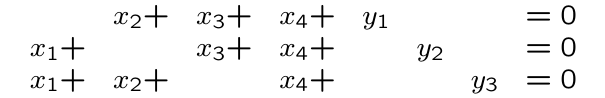
\includegraphics[width=0.45\textwidth]{img/hamming}
        \caption{Esempio con $k = 4$}
    \end{figure}
    Verrà poi inviata la sequenza $M = x_1x_2x_3x_4y_1y_2y_3$, il decodificatore calcolerà le 3 somme di controllo:
    \begin{itemize}[nosep]
        \item se sono tutte e tre uguali a 0, allora il decodificatore assume che non ci siano stati errori di comunicazione.
        \item se una somma è diversa da 0, allora il decodificatore assume che l'errore sia avvenuto sul bit di controllo.
        \item se 2 su 3 sono diverse da 0, allora il decodificatore assume che il bit scambiato è quello non presente nella terza somma.
        \item se sono tutti e tre diversi da 0, allora l'errore è nel quarto bit (presente in tutte le somme)
    \end{itemize}
    In questo caso avremo un \textbf{Tasso di informazione}: $\frac{k}{n} = \frac{k}{k +(k - 1)}$, solitamente migliore del codice ripetitivo.
    \item \textbf{Codice ISBM}:

    \begin{figure}[h]
        \centering
        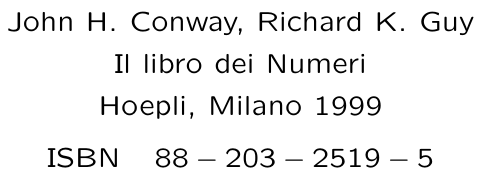
\includegraphics[width=0.35\textwidth]{img/isbm}
        \caption{International Standard Book Number}
    \end{figure}
    \begin{itemize}[nosep]
        \item 88: indica che il libro è stato pubblicato in Italia.
        \item 203: indica l'editore.
        \item 2519: identificativo di quel libro, dalla casa editrice.
        \item 5: cifra di controllo
    \end{itemize}
    Il numero complessivo è ammissibile come numero \textbf{ISBM} se la somma pesata $10 \cdot Y_10 + 9 \cdot Y_9 + ... + 1 \cdot Y_1$ da un risultato divisibile per 11. La cifra di controllo serve quindi per riconoscere errori di trasmissione, dovuti ad errori di scrittura o di comunicazione del numero ISBM.
\end{itemize}
\begin{flushleft}
    \textbf{Canale di Trasmissione}: Il canale binario simmetrico è uno dei modelli di trasmissione più utilizzati: accetta in ingresso e trasmette in usicta solo i caratteri $\mathbb{F} = \{0, 1\}$. \textbf{Probabilità cruda di errore} (\textbf{p}): è la probabilità con la quale, un bit entrato nel canale viene trasformato dal rumore nel bit complementare. Quindi, in una parola $x_1x_2...x_m$ avvengono $t$ errori con una probabilità pari:
    
    {\centering
        \fcolorbox{red}{white}{$(1 - p)^{m - t} \cdot p^t$}.
    \par}
\end{flushleft}

\newpage
\subsection{Interleaving}
\begin{flushleft}
    Si è supposto che i disturbi coinvolgano i caratteri in maniera indipendente, tuttavia, in realtà se un carattere viene alterato, allora è più facile che anche quelli vicini a lui vengano alterati. Il metodo di \textit{interleaving} è efficace control scrosci di errori (\textbf{burst errors}), che non siano troppo lunghi.

    \textcolor{orange}{\textbf{Esempi}} \\
    Data la sequenza da trasmettere: $10 \; 00 \; 01 \; 11 \; 11 \; 11 \; 01 \; 10 \; 00 \; 00 \; 10 \; 10 \; ...$
    Adottando il codice binario di lunghezza 5:$x_1x_2y_1y_2y_3$, dove $y_1 = x_1$, $y_2 = x_2$ e $y_3 = x_1 + x_2$, otteniamo delle parole che, memorizzate a gruppi di 4 creano delle matrici:

    \begin{figure}[h]
        \centering
        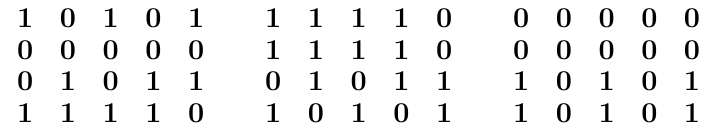
\includegraphics[width=0.45\textwidth]{img/interleaving_1}
    \end{figure}
    Il contenuto di tali matrici viene inviato colonna per colonna. Supponiamo che avvengano dei disturbi ai bit: 3, 5, 6, 39, 40, 41, 42, 59 e 60. Quindi il messaggio letto dal decodificatore sarà:

    \begin{figure}[h]
        \centering
        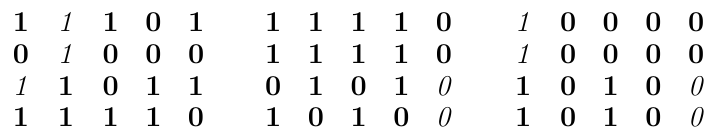
\includegraphics[width=0.45\textwidth]{img/interleaving_2}
    \end{figure}
    Riesce a decodificare correttamente i bit, perchè ogni riga ha al massimo 1 errore. I vantaggi dell'interleaving, tuttavia, si pagano con una maggiore complessità per la comunicazione e con dei ritardi nella trasmission dei dati.

    \textbf{Conclusioni}: un buon algoritmo di decodificazione, oltre a correggere un alto numeri di errori di trasmissione, deve essere facile da implementare. Una regola aurea adottata è quella di cercare codici con un alto grado di simmetria (ovver che abbiamo un \textbf{gruppo di automorfismi} molto ricco).
\end{flushleft}
\chapter{Calcolo Combinatorio}
Per scegliere le strutture combinatorie elementari coinvolte in un problema, occorre rispondere a due domande:
\begin{itemize}[nosep]
    \item l'\textbf{ordine} degli elementi è rilevante oppure no?
    \item gli elementi si possono \textbf{ripetere} oppure no?
\end{itemize}

\section{Strutture Combinatorie Elementari}
\begin{enumerate}[nosep]
    \item una \textbf{disposizione semplice} di $n$ oggetti a $k$ a $k$ con $k \leq n$ è una $k$-upla ordinata di $k$ oggetti distinti scelti tra gli $n$ dati (\textbf{non} si tiene conto dell'\textbf{ordine}, \textbf{non} si \textbf{ripetono} gli elementi).
    \begin{boxA}
        Il numero di disposizioni semplici è \fcolorbox{red}{white}{$D(n; k) = n \cdot (n - 1) \cdot ... \cdot (n - k + 1)$} \\
        \textcolor{orange}{\textbf{Esempio}}: In un collegio ci sono 10 professori, in quanti modi possono essere scelti \textit{presidente}, \textit{vicepresidente} e \textit{segretario}
        
        {\centering
            $D_{10, 3} = 10 \cdot 9 \cdot 8$
        \par}
    \end{boxA}
    \item una \textbf{disposizione con ripetizione} di $n$ oggetti a $k$ a $k$ è una $k$-upla ordinata di $k$ (non necessariamente distinti) scelti tra $n$ dati (si tiene conto dell'\textbf{ordine}, si possono \textbf{ripetere} gli elementi).
    \begin{boxA}
        Il numero di disposizioni con ripetizioni di $n$ oggetti a $k$ a $k$ è: \fcolorbox{red}{white}{$D^R(n; k) = n^k$} \\
        \textcolor{orange}{\textbf{Esempio}}: In un collegio ci sono 10 professori, in quanti modi posso scegliere i tutor per i 3 vincitori (un professore può essere tutor di più professori)

        {\centering
            $D^R_{10,3} = 10^3$
        \par}
    \end{boxA}
    
    \newpage
    \item una \textbf{permutazione} di $n$ oggetti è una $n$-upla ordinata i cui elementi sono tutti gli $n$ oggetti (è una disposizione semplice di $n$ oggetti a $n$ a $n$). Il numero di permutazioni di $n$ oggetti è:
    
    {\centering
        \fcolorbox{red}{white}{$P(n) = n!$}
    \par}
    
    \item una \textbf{combinazione semplice} di $n$ oggetti a $k$ a $k$ (con $k \leq n$) è un sottoinsieme di $k$ oggetti distinti scelti tra gli $n$ dati (in questo caso \textbf{non} conta l'\textbf{ordine} e \textbf{non} posso ripetere gli elementi).
    \begin{boxA}
        Il numero di combinazioni semplici di $n$ oggetti a $k$ a $k$ è il ``\textit{coefficente binomiale}'' di $n$ su $k$: \fcolorbox{red}{white}{$C(n; k) = \binom{n}{k} = \frac{n!}{k! \cdot (n - k)!}$} \\
        \textcolor{orange}{\textbf{Esempio}}: In un collegio di sono 10 professori, in quanti modi posso scegliere 3 professori per la commissione

        {\centering
            $C_{10,3} = \binom{10}{3} = \frac{10!}{3! \cdot (10 - 3)!} = \frac{10!}{3! \cdot 7!} = \frac{10 \cdot 9 \cdot 8 \cdot \cancel{7!}}{3! \cdot \cancel{7!}} = \frac{10 \cdot 9 \cdot 8}{3!}$
        \par}
    \end{boxA}
\end{enumerate}

\begin{flushleft}
    \textbf{Definizione}: un \textbf{Multinsieme} di cardinalità $k$ è una collezione di oggetti, ciascuno ripetuto con una data molteplicità, in modo che la somma delle molteplicità sia pari a $k$. 

    \textbf{Definizione}: una \textbf{combinazione con ripetizione} di $n$ oggetti a $k$ a $k$ è una collezione di $k$ oggetti (non necessariamente distinti) scelti tra gli $n$ oggetti dati (ovvero: è un \textit{sotto-insieme} di cardinalità $k$ dell'insieme di $n$ oggetti dati). Il numero di combinazioni con ripetizioni di $n$ oggetti a $k$ a $k$ è:

    {\centering
        \fcolorbox{red}{white}{$C^R(n; k) = \binom{n + k - 1}{k}$}
    \par}

    \textbf{N.B.}: la differenza tra \textbf{insieme} e \textbf{multinsieme} è che un insieme a tutti gli elementi distinti, mentre un multinsieme ammette anche elementi ripetuti.
    \begin{boxA}
        \textcolor{olive}{\textbf{Dimostrazione}}: consideriamo $\mathbb{N}_n = \{1, 2, ..., n - 1\}$, per avere una combinazione con ripetizione di $k$ elementi in $\mathbb{N}_n$, devo scegliere:

        {\centering
            $1 \leq a_1 \leq a_2 \leq ... \leq a_{k - 1} \leq a_k \leq n$
        \par}
        Osservando le combinazioni semplici, cioè con elementi tutti distinti: \newline
        $1 \leq a_1 < a_2 + 1 \leq a_3 + 1 \leq ... \leq n + 1$ \newline
        $1 \leq a_1 < a_2 + 1 < a_3 + 1 + 1 \leq ... \leq n + 1 + 1$ \newline
        $\cdots$ \newline
        $1 \leq a_1 < a_2 + 1 < a_3 + 2 < ... < a_{k - 1} + (k - 2) < a_k + (k - 1) \leq n + (k - 1)$

        Questo implica che, svegliere $k$ elementi con ripetizione tra $1$ e $n$, è come scegliere $k$ elementi distinti tra $1$ e $n + (k - 1)$, quindi il numero di combinazioni con ripetinizioni di $n$ elementi a $k$ a $k$ è: $C^R(n; k) = C^R(n + k -1; k) = \binom{n + k - 1}{k}$ 
    \end{boxA}
    \begin{boxA}
        \textcolor{orange}{\textbf{Esempi}}
        \begin{enumerate}[nosep]
            \item consideriamo la parola ``discreta'', quanti sono gli anagrammi (anche senza senso). Consideriamo che l'insieme $\mathbb{S} = \{d, i, s, c, r, e, t, a\}$ ogni suo elemento ha \textbf{molteplicità} uno, quindi l'esercizio si risolve con una \textbf{permutazione}:

            {\centering
                $P_3 = 8!$
            \par}
            \item consideriamo la parola ``matematica'', quanti sono gli anagrammi (anche senza senso). Consideriamo l'insieme $\mathbb{S} = \{m, a, t, e, i,c\}$ in questo caso non tutti gli elementi dell'insieme hanno molteplicità uno, ad esempio, $a$ ha molteplicità tre. Quindi dobbiamo utilizzare una \textbf{Permutazione su un multinsieme}.
        \end{enumerate}
    \end{boxA}

    Una \textbf{Permutazione su un Multinsieme} di cardinalità $n$, i cui elementi hanno rispettivamente molteplicità $k_1, ..., k_r$ (con $r \geq 1, \; k_1 \geq 1 \; \forall i \in \{1, ..., r\}$ e tali che $\sum_{i = 1}^r k_i = n$) è una $n$-upla ordinata i cui elementi sono tutti gli $n$ oggetti (non tutti distinti) del multinsieme. Il numero di permutazioni su un multinsieme è pari:

    {\centering
        \fcolorbox{red}{white}{$P^R(n; k_1, k_2, ..., k_r) = \frac{n!}{k_1 \cdot k_2 \cdot ... \cdot k_r}$}
    \par}
\end{flushleft}

\section{Principi Fondanti del Calcolo Combinatorio}

\begin{itemize}[nosep]
    \item \textbf{Principio della Somma}: dati due insiemi finiti e disgiunti $A$ e $B$, allora: \fcolorbox{red}{white}{$\# (A \cup B) = \# A + \# B$}
    \item \textbf{Principio Generalizzato della Somma}: dati $n$ insimi finiti $A_1, A_2, ..., A_n$ con $A_i \cap A_j = \emptyset \; \forall i \neq j \; i,j \in \mathbb{N}_n$, allora: \fcolorbox{red}{white}{$\# (\underset{i \in \mathbb{N}_n}{\bigcup} A_i) = \underset{i \in \mathbb{N}_n}{\sum}\# A_i$}
    \item \textbf{Principio del Prodotto}: dati due insiemi finiti $A$ e $B$, allora: \fcolorbox{red}{white}{$\# (A \times B) = \# A \cdot \# B$}
    \item \textbf{Principio Generalizzato del Prodotto}: dati $n$ insimei finiti $A_1, A_2, ..., A_n$ allora: \\
    \fcolorbox{red}{white}{$\# (A_1 \times A_2 \times ... \times A_n) = \underset{i \in \mathbb{N}_n}{\prod} \# A_i$}
    \item \textbf{Principio di Inclusione/Esclusione}: siano $A$ e $B$ insiemi finiti, con $\# A = n$ e $\# B = m$, allora: \fcolorbox{red}{white}{$\# (A \cup B) = \# A + \# B - \# (A \cap B)$}

    \begin{center}
        \begin{minipage}[t]{0.1\textwidth}
            \centering
            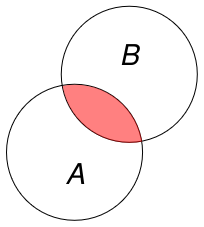
\includegraphics[width=\textwidth]{img/inc_escl_1}
        \end{minipage}
        \hfill
        \begin{minipage}[t]{0.8\textwidth}
            \begin{boxA}
                \textcolor{olive}{\textbf{Dimostrazione}}: consideriamo l'unione disgiunta: $A \cup B = A \cup (B - A)$ \\
                $\Rightarrow \# (A \cup B) = \# A + \fcolorbox{red}{white}{$\# (B - A)$}$, mentre B lo posso vedere come: \\
                $B = (B - A) \cup (A \cap B) \rightarrow \# B = \# (B - A) + \# (A \cap B)$ Quindi avremo \\
                $\fcolorbox{red}{white}{$\# (B - A)$} = \# B - \# (A \cap B)$, sostituendo 
                
                {\centering
                    \fcolorbox{red}{white}{$\# (A \cup B) = \# A + \# B - \# (A \cap B)$}
                \par}
            \end{boxA}
        \end{minipage}
    \end{center}

    \newpage
    \item \textbf{Principio di Inclusione/Esclusione con tre Insiemi}: se $A$, $B$ e $C$ sono insiemi finiti, allora: \fcolorbox{red}{white}{$\# (A \cup B \cup C) = \# A + \# B + \# C - \# (A \cap B) - \# (A \cap C) - \# (B \cap C) + \# (A \cap B \cap C)$}

    \begin{figure}[h]
        \centering
        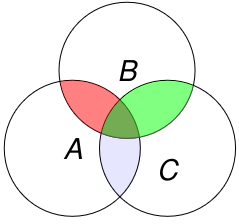
\includegraphics[width=0.1\textwidth]{img/inc_escl_2}
    \end{figure}
    \begin{boxA}
        \textcolor{olive}{\textbf{Dimostrazione}}
        \begin{align*}
            \# (A \cup B \cup C) &= \# [(A \cup B) \cup C] = \# (A \cup B) + \# C - \# [(A \cup B) \cap C] \\
            &= \# (A \cup B) + \# C - \# [(A \cap C) \cup (B \cap C)] \\
            &= \# A + \# B - \# (A \cap B) + \# C - \# (A \cap C) - \# (B \cap C) + \# (A \cap B \cap C) \\
            &= \underline{\# A + \# B + \# C - \# (A \cap B) - \# (A \cap C) - \# (B \cap C) + \# (A \cap B \cap C)}
        \end{align*}
    \end{boxA}
\end{itemize}

\begin{flushleft}
    \textbf{Formula di Da Silva}: Se $A_1, A_2, ..., A_n$ sono insiemi finiti, allora:

    {\centering
        $\# (\underset{i \in \mathbb{N}_n}{\bigcup} A_i) = \underset{I \subseteq \mathbb{N}_n, \; I \neq \emptyset}{\sum} (-1)^{\# I - 1} \cdot \# (\underset{i \in I}{\bigcap} A_i)$
    \par}
    Generalizzando per $n$ insiemi finiti: vengono aggiunte le cardinalità singole, si tolgono quelle a due a due, si aggiungono quelle a tre a tre, si tolgono quelle a quattro a quattro, e via dicendo. In questo modo avremo $2^n - 1$ addendi.
\end{flushleft}
\chapter{Relazioni Ricorsive}

\begin{flushleft}
    Una successione $\{a_n\}_{n \in \mathbb{N}}$ a valori interi può essere data in due forme differenti:
    \begin{itemize}[nosep]
        \item per \textbf{elencazione}: $\{a_0, a_1, ..., a_i, ...\}$, con $a_i \in mathbb{Z} \; \forall i \in \mathbb{N}_0$
        \item in \textbf{forma chiusa}: $a_n = f(n)$, con $f : \mathbb{N}_0 \mapsto \mathbb{Z}$, $f$ è un'\textbf{applicazione}
    \end{itemize}

    \textbf{Successioni Definite per Ricorsione}: una successione è definita \textbf{ricorsivamente} (ovvero tramite una \textbf{relazione ricorsiva}) se ogni termine della successione è espresso in funzione dei termini precedenti, e se sono noti un certo numero di termini iniziali che permettano di individuare univocamente la successione.

    Risolvere una \textit{relazione ricorsiva} significa ottenere una definizione in forma chiusa della successione stessa.

    \begin{boxA}
        \textcolor{orange}{\textbf{Esempio}} \\
        $\begin{cases}
            a_n = 3 \cdot a_{n - 1} \quad n > 1 \; \text{(relazione ricorsiva)} \\
            a_1 = 3 \qquad \qquad \qquad \;\; \text{(condizione iniziale)}
        \end{cases}$ \\
        definisce univocamente la successione \fcolorbox{orange}{white}{$\{a_n\}_{n \in \mathbb{N}} = \{3, 3^2, 3^3, ...\}$} che si può rappresentare in forma chiusa come:

        {\centering
            $a_n = 3^n \; \forall n \in \mathbb{N}$
        \par}
    \end{boxA}

    Una relazione ricorsiva si dice di \textbf{ordine \textit{k}} se il generico elemento $a_n$ della successione è dato in funzione di $k$ elementi che lo precedono. La relazione ricorsiva determinerà univocamente una successione, noti i $k$ elementi iniziali della successione

    Una relazione ricorsiva di ordine $k$ si dice \textbf{lineare} se viene rappresentata come:

    {\centering
        $a_n = b_{n - 1}(n) \cdot a_{n - 1} + b_{n - 2}(n) \cdot a_{n - 2} + ... + b_{n - k}(n) \cdot a_{n - k} + d(n)$
    \par}
    dove i $b_{n - i}(n) \; i \in \mathbb{N}$ sono delle funzioni (non necessariamente lineari) che determinano i coefficienti $a_{n - i} \; i \in \mathbb{N}$ mentre $d(n)$ è il termine noto (può non essere lineare).

    Una relazione ricorsiva \textit{lineare} si dice \textbf{omogenea} se il termine noto è nullo, ovvero $d(n) = 0$

    Una relazione ricorsiva \textit{lineare} si dice a \textbf{coefficienti costanti} se le funzioni coefficienti [$b_{n - i}(n) \; i \in \mathbb{N}$] sono funzioni costanti, ovvero $b_{n - i}(n) = \alpha_i$, con $\alpha_i$ costante $\forall i$ e viene rappresentata:

    {\centering
        $a_n = \alpha_1 \cdot a_{n - 1} + \alpha_2 \cdot a_{n - 2} + ... + \alpha_k \cdot a_{n - k} + d(n)$
    \par}
\end{flushleft}

\section{Relazioni Ricorsive Lineari del 1$^\circ$ Ordine}

\begin{flushleft}
    \textbf{Relazioni ricorsive lineari omogenee del I ordine a coefficienti costanti}: la successione definita da: 

    {\centering
        $\begin{cases}
            a_n = b \cdot a_{n - 1} \quad \forall n > m \\
            a_m = c
        \end{cases}$
    \par}
    ha come forma chiusa: \fcolorbox{red}{white}{$a_n = c \cdot b^{n - m} \; \forall n \geq m$}

    \begin{boxA}
        \textcolor{olive}{\textbf{Dimostrazione}}: si dimostra per \textbf{induzione} \newline
        \textcolor{red}{\textbf{Passo Iniziale}}: poniamo $n = m$ allora avremo che: 

        {\centering
            $a_n = c \cdot b^{m - m} = c \cdot b^0 = c$
        \par}
        abbiamo dimostrato le condizioni di partenza della relazione ricorsiva.

        \textcolor{red}{\textbf{Passo Induttivo}}

        {\centering
            \begin{minipage}[t]{0.45\textwidth}
                \centering
                \textbf{Hp.} $a_{n - 1} = c \cdot b^{n - 1 - m}$
            \end{minipage}
            \begin{minipage}[t]{0.45\textwidth}
                \centering
                \textbf{Th.} $a_n = c \cdot b^{n - m}$
            \end{minipage}
            $a_n = b \cdot a_{n - 1} = b \cdot c \cdot b^{n - 1 - m} = c \cdot b^{n - m}$
        \par}

        \textcolor{orange}{\textbf{Esempio}}

        {\centering
            $\begin{cases}
                a_n = 3a_{a - 1} \\
                a_0 = 2
            \end{cases}$
            $\Rightarrow a_n = 2 \cdot 3^{n - 0} = 2 \cdot 3^n$
        \par}
    \end{boxA}
    \textbf{Relazioni ricorsive lineari omogenee del I ordine a coefficienti non costanti}: la successione definita da:

    {\centering
        $\begin{cases}
            a_n = b(n) \cdot a_{n - 1} \quad \forall n > m \\
            a_m = c
        \end{cases}$
    \par}
    ha come forma chiusa \fcolorbox{red}{white}{$a_n = c \cdot \underset{i = 1}{\overset{n - m}{\prod}} b (m + i) \; \forall n \geq m$}. La forma chiusa può essere dimostrata per \textbf{induzione}, in perfetta analogia al caso precedente:
\end{flushleft}

\newpage
\begin{flushleft}

    \textbf{Relazioni ricorsive lineari del I ordine non omogenee a coefficienti costanti}: la successione definita da:

    {\centering
        $\begin{cases}
            a_n = b \cdot a_{n-1} + d(n) \quad \forall n > m \\
            a_m = c
        \end{cases}$
    \par}
    ha come forma chiusa: \fcolorbox{red}{white}{$a_n = b^{n-m} \cdot [c + \underset{i = 1}{\overset{n-m}{\sum}} d(m + i) \cdot b^{-i}] \; \forall n \geq m$}

    \begin{boxA}
        \textcolor{olive}{\textbf{Dimostrazione}}: la forma chiusa viene dimostrata sempre per \textbf{induzione}

        \textcolor{red}{\textbf{Passo Iniziale}}: poniamo $n = m$

        {\centering
            $a_n = b^{m-m} \cdot [c + \underset{i = 1}{\overset{m-m}{\sum}} d(m + i) \cdot b^{-i}] = [c + \cancel{\underset{i = 1}{\overset{0}{\sum}} d(m + i) \cdot b^{-1}}] = c$
        \par}

        \textcolor{red}{\textbf{Passo Induttivo}}

        {\centering
            \begin{minipage}[t]{0.45\textwidth}
                \centering
                \textbf{Hp.} \\
                $a_{n - 1} = b^{n-1-m} \cdot [c + \underset{i=1}{\overset{n-1-m}{\sum}} d(m + i) \cdot b^{-i}]$
            \end{minipage}
            \begin{minipage}[t]{0.45\textwidth}
                \centering
                \textbf{Th.} \\
                $a_n = b^{n-m} \cdot [c + \underset{i = 1}{\overset{n-m}{\sum}} d(m + i) \cdot b^{-i}]$
            \end{minipage}
        \par}

        $a_n = b \cdot a_{n-1} + d(n) = b \cdot b^{n-1-m} [c + \underset{i=1}{\overset{n-1-m}{\sum}} d(m+i) \cdot b^{-1}] + d(n) \cdot \fcolorbox{brown}{white}{$(b^{n-m} \cdot b^{-(n-m)})$}$ moltiplico e divido per $b^{n-m}$ in modo da poter raccogliere al primo addendo.
        \begin{align*}
            a_n &= b \cdot b^{n-1-m} [c + \underset{i=1}{\overset{n-1-m}{\sum}} d(m+i) \cdot b^{-1}] + d(n) \cdot (b^{n-m} \cdot b^{-(n-m)}) \\
            &= b^{n-m} [c + \underset{i=1}{\overset{n-1-m}{\sum}} d(m+i) \cdot b^{-1}] + d(n) \cdot (b^{n-m} \cdot b^{-(n-m)}) \\
            &= b^{n-m} \cdot \{[c + \underset{i=1}{\overset{n-1-m}{\sum}} d(m+i) \cdot b^{-1}] + \fcolorbox{blue}{white}{$d(n) \cdot b^{-(n-m)}$}\} \\
            &= b^{n-m} \cdot [c + \underset{i = 1}{\overset{n-m}{\sum}} d(m + i) \cdot b^{-i}]
        \end{align*}
        Il valore \fcolorbox{blue}{white}{$d(n) \cdot b^{-(n-m)}$} posso portarlo dentro alla sommatoria in modo da poter ottenere e dimostrare la tesi.
    \end{boxA}
\end{flushleft}

\begin{boxA}
    \textcolor{orange}{\textbf{Esempio - Torre di Hanoi}}: bisogna spostare $n$ dischi di diametro crescente, in modo da riottenere la torre sull'ultima colonna. \textbf{Regole}: ad ogni passo si può spostare un solo disco, un disco non può mai essere spostato sopra ad uno di diametro inferiore.
    
    \begin{center}
        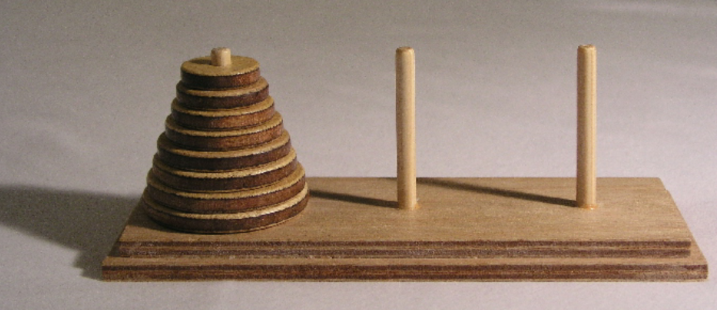
\includegraphics[width=0.65\textwidth]{img/hanoi}
    \end{center}

    Per spostare il generico $n$-esimo disco: $H_n = H_{n-1} + 1 + H_{n-1} = 2 \cdot H_{n-1} + 1$. Quindi la nostra relazione ricorsiva sarà:
    $H(n) = \begin{cases}
        H_n = 2 \cdot H_{n-1} + 1 \\
        H_1 = 1
    \end{cases}$
    
    \begin{align*}
        H(n) &= 2^{n-1} [1 + \underset{i=1}{\overset{n-1}{\sum}}1 \cdot 2^{-i}] \\
        &= 2^{n-1} [\underset{i=0}{\overset{n-1}{\sum}}1 \cdot 2^{-i}] \\
        &= 2^{n-1} \cdot \frac{1-(\frac{1}{2})^n}{1-\frac{1}{2}} \\
        &= 2^n \cdot (1 - \frac{1}{2^n}) = 2^n - 1 \; \text{mosse}
    \end{align*}
\end{boxA}

\begin{flushleft}
    \textbf{Relazioni ricorsive lineri non omogenee del I ordine a coefficienti non costanti}: la successione definita da:

    {\centering
        $\begin{cases}
            a_n = b(n) \cdot a_{n-1} + d(n) \quad \forall n > m \\
            a_m = c
        \end{cases}$
    \par}
    ha come forma chiusa: \fcolorbox{red}{white}{$a_n = \underset{i=1}{\overset{n-m}{\prod}} b(m+i) \cdot [c + \underset{i=1}{\overset{n-m}{\sum}} d(m+i) \cdot \underset{j=1}{\overset{i}{\prod}} \frac{1}{b(m+j)}] \; \forall n \geq m$}. La forma chiusa può essere verificata per \textbf{induzione} come il caso a \textit{coefficienti costanti}.
\end{flushleft}

\newpage
% PAGINA VUOTA
%\clearpage\null\thispagestyle{empty}\clearpage
%\appendix
%\appendixpage
%\addappheadtotoc

%\clearpage\null\thispagestyle{empty}\clearpage


%\listoffigures


\begin{flushleft}
\bibliographystyle{plain}
\bibliography{sections/references} 
\end{flushleft}

\end{document}
